\documentclass[conference]{IEEEtran}
\IEEEoverridecommandlockouts
% The preceding line is only needed to identify funding in the first footnote. If that is unneeded, please comment it out.
\usepackage{cite}
\usepackage{amsmath,amssymb,amsfonts}
\usepackage{algorithmic}
\usepackage{graphicx}
\usepackage{textcomp}
\usepackage{xcolor}
\usepackage{hyperref}
\def\BibTeX{{\rm B\kern-.05em{\sc i\kern-.025em b}\kern-.08em
    T\kern-.1667em\lower.7ex\hbox{E}\kern-.125emX}}
\begin{document}

\title{COM3240 Assignment Report}

\author{\IEEEauthorblockN{Jiacong Wu}
% \IEEEauthorblockA{\textit{dept. name of organization (of Aff.)} \\
% \textit{name of organization (of Aff.)}\\
% City, Country \\
% email address or ORCID}
}

\maketitle

\section{Introduction}
In this assignment, we aim to explore how the SARSA algorithm perform, compared to Q-learning, for a reinforcement learning application to a modified game of chess on a 4x4 board, where agent aims to checkmate the opponent given an initial, random, legal board state.

\section{Task 1 - Q-Learning and SARSA}
In Q-learning, for an agent in state $s$, taking an action $a$ based on a behaviour/action selection policy, it receives reward $r$ and moves to a new state $s'$. We obtain the expected reward $Q(s',a')$ from the new state and a new action $a'$, based on the target policy (in the case of Q-learning, this target policy is always greedy \cite{sarsa yt}), which contributes to the target Q value in the update of the Q-value of a state-action pair using equation \ref{eq:q_learning_update_rule}

\begin{equation}
    Q(s,a) = Q(s,a) + \eta(r + \max_{a'}\gamma Q(s',a') - Q(s,a))
    \label{eq:q_learning_update_rule}
\end{equation}

\begin{itemize}
    \item $\gamma$ is the discount factor $0 < \gamma < 1$, adjusted depending on how much importance to put on the immediate reward and future reward. For $\gamma = 0$, the agent will only consider the immediate reward, while a factor approaching 1 will make it strive for a long-term high reward \cite{sarsa}.
    \item $\eta$ is the learning rate/step size, which is used to control the speed of learning.
\end{itemize}

The SARSA (State-action-reward-state-action) algorithm is a slightly modified version of the Q-learning algorithm, in the difference being it uses the action $a'$ selected by the behaviour policy to obtain the expected reward $Q(s',a')$ in the update of the Q-value of a state-action pair using equation \ref{eq:sarsa_q_update_rule}, instead of using a fixed greedy target policy as with Q-learning

\begin{equation}
    Q(s,a) = Q(s,a) + \eta(r + \gamma Q(s',a') - Q(s,a))
    \label{eq:sarsa_q_update_rule}
\end{equation}

And obviously, with SARSA's approach we will have the advantage of being able to use a non-greedy behaviour policy for obtaining the expected reward, which allows the algorithm to explore a range of different solutions, and not be potentially stuck in a local optimal solution as with Q-learning's greedy approach. 

\section{Task2 - Implementing SARSA}
We wrote the code to forward inference of the neural network to obtain the Q-value for each action, shown in Figure \ref{fig:forward_inference} (implementation details/code are listed in the Appendix section). The RELU activation function for the output weighted sums from the hidden layers, instead of a sigmoid function. The advantage of using RELU is that it reduces the likelihood of the vanishing gradient problem\cite{relu advantage}, arising from gradient-based such as backpropagation which is what we used to train the neural network\cite{vanishing gradient problem}. The vanishing gradient problem is when the gradient of the loss function approaches 0, causing the weights to not be updated, and therefore the neural network will fail to learn anything.

We proceed to implement the behaviour/action policy in Figure \ref{fig:behaviour_policy}. The behaviour policy is epsilon-greedy, where the agent will take a random action \texttt{a\_agent} from the array of legal actions \texttt{a}, with probability $\epsilon$, and take the greedy action with probability $1 - \epsilon$. If after taking the action, we haven't reached the terminal state, another action \texttt{a\_agent2} will be taken from the list of next legal actions, resulted taking the previous action as shown in Figure \ref{fig:target_policy_sarsa}. This is chosen according to a target policy, which is the same as the behaviour policy in the case of SARSA.

A factor of the Q-value corresponding to the next action is added to the target reward to incorporate future reward. In the case of choosing an action that reaches a terminal state (checkmate or stalemate), no future action can be taken, therefore no future is incorporated. An error signal, which is the difference between the target and actual output, is computed in order to perform backpropagation. The weights are updated with the ADAM optimizer, which is a gradient descent optimization algorithm that helps us achieve convergence much quicker. When updating the weights for the last layer \texttt{W2}, we made sure we are only updating the weights corresponding to the action taken and not all the weights. We also implemented a function in Figure \ref{fig:exponential_moving_average} for computing the exponential moving averages for the data we collected, for the accumulated reward and number of moves taken during each episode.

I found out that using a learning rate $\eta$ of 0.00035, which is 10 times smaller than the suggested value, gave the best average reward of around 0.85 at the end of 20000 episodes. As I proceed to train with more episodes, I found out that the average reward started to decrease instead of converging to a value 1 as one might expect, shown in Figure \ref{fig:gamma_0_85}.

\begin{figure}[htbp]
\centerline{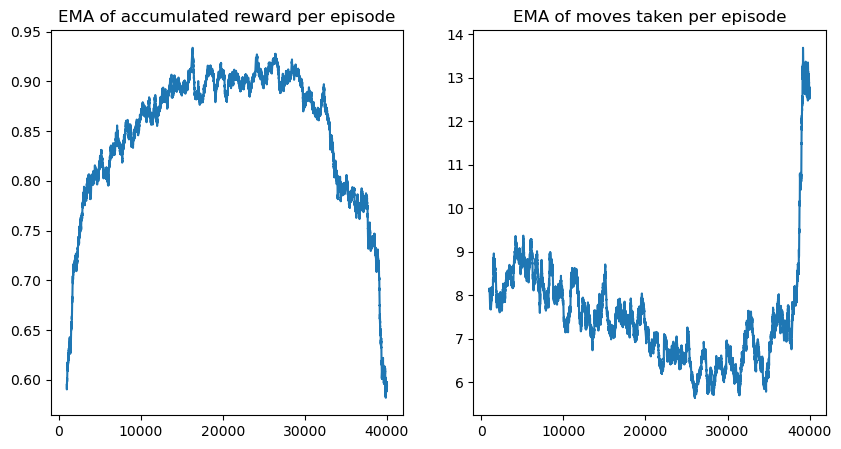
\includegraphics[width=0.5\textwidth]{images/gamma_0_85.png}}
\caption{EMA of data recorded, with $\eta=0.00035$, $\gamma=0.85$, $N\_episodes=40000$}
\label{fig:gamma_0_85}
\end{figure}

This issue was addressed by using a discount factor $\gamma$ of 0.9, achieving a stable convergence trend in Figure \ref{fig:gamma_0_90} below.

\begin{figure}[htbp]
\centerline{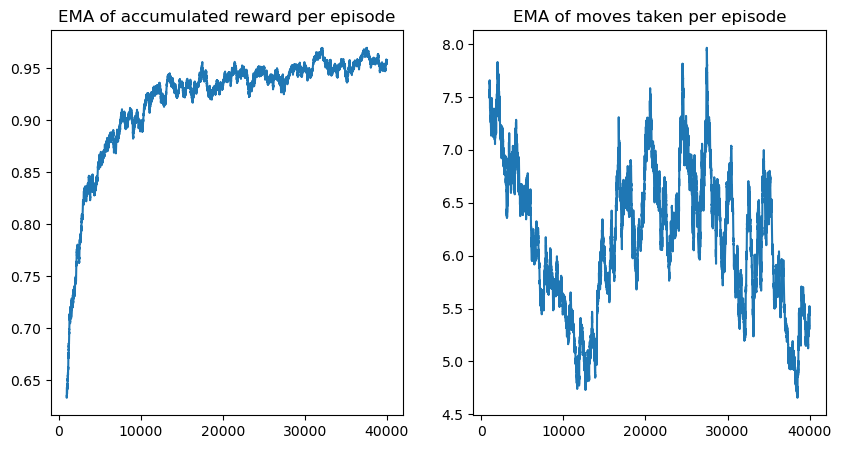
\includegraphics[width=0.5\textwidth]{images/gamma_0_90.png}}
\caption{EMA of data recorded, with $\eta=0.00035$, $\gamma=0.9$, $N\_episodes=40000$}
\label{fig:gamma_0_90}
\end{figure}

\section{Task 3 - Varying $\gamma$ and $\epsilon$ via $\beta$}
\subsection{Varying $\gamma$}
$\gamma$ is the discount factor controlling the importance of future rewards. A higher $\gamma$ value will make the agent strive for a long-term high reward, while a lower $\gamma$ value will make the agent focus on the immediate reward. In the case of the modified chess game, a higher $\gamma$ value will make the agent focus on the long-term reward of checkmating the opponent and therefore incorporating long-term planning behaviour. While a lower $\gamma$ value will make the agent focus on immediate rewards such as threatening the opponent's king. We found out previously during implementation that a $\gamma$ of 0.9 gave the best results, increasing or decreasing beyond that value resulted in unstablity during training. This resulted in the average reward to drop and the number of moves taken to increase.

\subsection{Varying $\epsilon$ via $\beta$}
$\epsilon$ is the probability of the agent taking a random action, instead of a greedy action by choosing the action that corresponds to the highest Q-value. A higher $\epsilon$ value will make the agent more likely to take a random action, while a lower $\epsilon$ value will make the agent more likely to take the greedy action, which will allow the agent to exploit the current best solution.

$\beta$ is a parameter that sets how quickly the value of $\epsilon$ is decaying. After each episode, $\epsilon$ is set using equation \ref{eq:epsilon_decay}, where $\epsilon_0$ is the initial probability and $n$ is the episode number.

\begin{equation}\label{eq:epsilon_decay}
    \epsilon_n = \frac{\epsilon_0}{1 + \beta * n}
\end{equation}

\section{Task 4 - Implementing Q-Learning}


\begin{thebibliography}{00}
\bibitem{sarsa yt} P. Porwal, "SARSA (State Action Reward State Action) Learning - Reinforcement Learning - Machine Learning" YouTube. \url{https://www.youtube.com/watch?v=FhSaHuC0u2M&ab_channel=PankajPorwal} (Accessed: April 6, 2023)

\bibitem{sarsa} "State–action–reward–state–action", Wikipedia. \url{https://en.wikipedia.org/wiki/State%E2%80%93action%E2%80%93reward%E2%80%93state%E2%80%93action} (Accessed: April 6, 2023)

\bibitem{relu advantage} DaemonMaker, "What are the advantages of ReLU over sigmoid function in deep neural networks?" Stack Overflow. \url{https://stats.stackexchange.com/questions/126238/what-are-the-advantages-of-relu-over-sigmoid-function-in-deep-neural-networks} (Accessed: May 16, 2023)

\bibitem{vanishing gradient problem} "The Vanishing Gradient Problem" Great Learning. \url{https://www.mygreatlearning.com/blog/the-vanishing-gradient-problem/} (Accessed: May 16, 2023)

\end{thebibliography}

\appendix

\begin{figure}[htbp]
\centerline{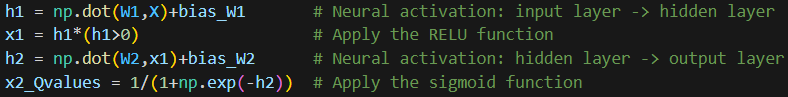
\includegraphics[width=0.45\textwidth]{images/forward_inference.png}}
\caption{Forward inference/neural activation of neural network to calculate Q-value for each action}
\label{fig:forward_inference}
\end{figure}

\begin{figure}[htbp]
\centerline{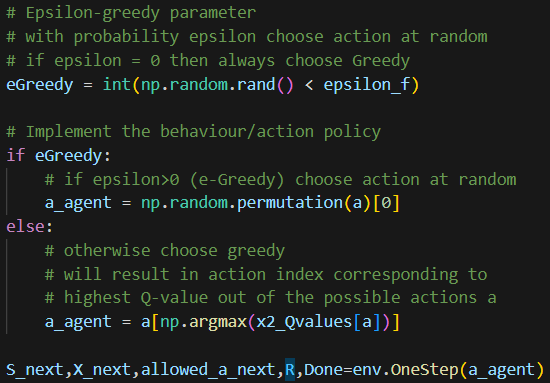
\includegraphics[width=0.45\textwidth]{images/behaviour_policy.png}}
\caption{Implementing epsilon-greedy behaviour policy}
\label{fig:behaviour_policy}
\end{figure}

\begin{figure}[htbp]
\centerline{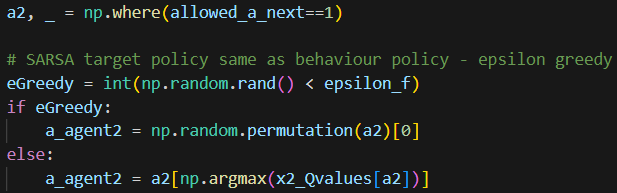
\includegraphics[width=0.45\textwidth]{images/target_policy_sarsa.png}}
\caption{Implementing epsilon-greedy target policy for SARSA}
\label{fig:target_policy_sarsa}
\end{figure}

\begin{figure}[htbp]
\centerline{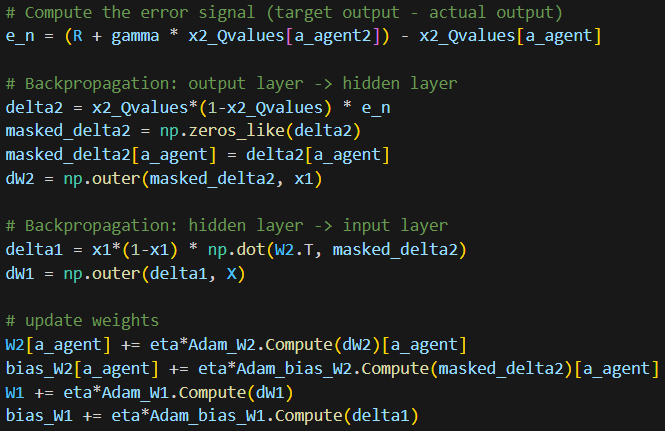
\includegraphics[width=0.45\textwidth]{images/backpropagation.png}}
\caption{Backpropagation and update weights with ADAM optimizer}
\label{fig:backpropagation}
\end{figure}

\begin{figure}[htbp]
\centerline{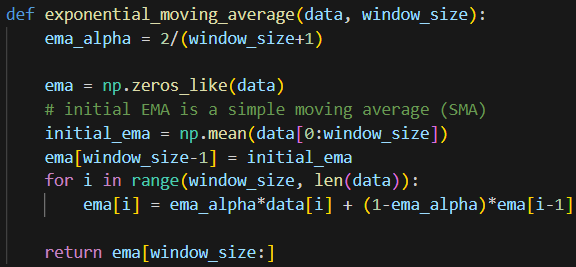
\includegraphics[width=0.45\textwidth]{images/ema.png}}
\caption{Function for computing exponential moving averages}
\label{fig:exponential_moving_average}
\end{figure}

\end{document}
